  \section{Hardware}
  Hardware implementering af \textit{The Cell Collector} består af enhedstest af hver komponent, med følgende dokumentation. Enhedstestene er lavet i den skrevne rækkefølge og integreret i samme. I dette afsnit vil der være kredsløbsdiagrammer, teori, beregninger og beskrivelser, hvilket er udarbejdet sideløbende med udviklingen af produktet. 
 	
 \subsection{Vægtcelle}
 For at kunne udnytte funktionen af en vægtcelle, skal opbygningen af denne forstås. En vægtcelle måler hvor meget vægt den udsættes for vægtcellen, der er brugt i projektet, består af strain gages koblet i en wheatstone bro. En strain gage bruges til at måle fysisk stræk eller kompression. Den er simpel i sin opbygning ved at består af en meget tynd elektrisk ledende tråd, som er ført frem og tilbage på et elastisk folie, hvilket er illustreret på \ref{fig:Strain gages}\footnote{billedet er hentet med tilladelse fra  \url{https://en.wikipedia.org/wiki/Strain_gauge}}. 
 \begin{figure}[H]
	\centering
	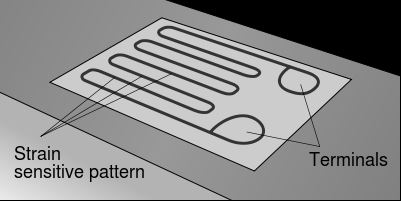
\includegraphics[width=0.5\textwidth]{billeder/Hardware/straingages1.JPG}
	\caption{illustration af strain gages}
	\label{fig:Strain gages}
\end{figure}
En strain gages modstand stiger ved stræk og falder ved kompression, dette kan beskrives ud fra formlen \ref{eq:modstandsformel}\citep{Websterbog}{s.47}
 \begin{align}
 R=\frac{\rho*L}{A}
 \label{eq:modstandsformel}
 \end{align}
 Hvor R=modstand, $\rho$=modstand per meter, L=længden og A=tværsnitsarealet. Der er mere til formlen en dette, bla. materiales egenskaber og temperatur. På vægtcellen er der fire strain gages, som er placeret på vægtcellen på denne måde som vist på figur \ref{fig:Loadcell1}. Strain gages R1 og R4 bliver strukket, hvor R2 og R3 på undersiden bliver skubbet sammen.
 
 Måden de er forbundet er vist på figur \ref{fig:loadcell2}, denne metode at koble modstande på kaldes en wheatstone bro\citep{ELengbog}{s.122}. mere specifikt for denne er også kendt som et full-bridge kredsløb\citep{AETbog}{s.76}. Forholdet mellem input spændingen og output spændingen kan beskrives, som vist ved formlen\ref{eq:fullbformel}
\begin{align}
 V_{out}=GF*V_{in}*\varepsilon
 \label{eq:fullbformel}
 \end{align}
 Hvor V$_{out}$=udgangssignalet, V$_{in}$=indgangsspændingen , GF=gages factor som er materialets egenskab og $\varepsilon$=strukket der er tilført til vægtcellen.

\begin{figure}[htbp] \centering
\begin{minipage}[b]{0.48\textwidth} \centering
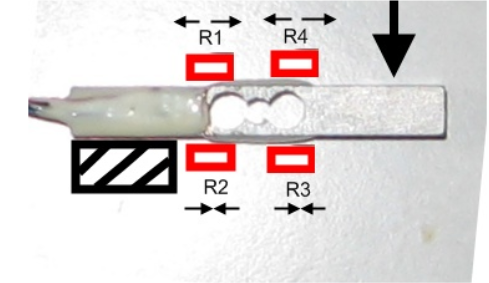
\includegraphics[width=1.00\textwidth]{billeder/Hardware/loadcell1.PNG} % Left picture
\end{minipage} \hfill
\begin{minipage}[b]{0.48\textwidth} \centering
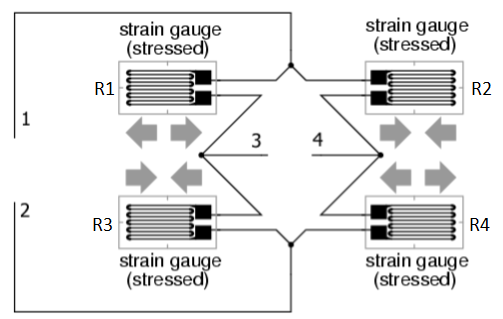
\includegraphics[width=1.00\textwidth]{billeder/Hardware/straingages2.PNG} % Right picture
\end{minipage} \\ % Captions og labels
\begin{minipage}[t]{0.48\textwidth}
\caption{Illustration af strain gages i loadcell på virkning} % Left caption and label
\label{fig:Loadcell1}
\end{minipage} \hfill
\begin{minipage}[t]{0.48\textwidth}
\caption{Illustration af koblingen strain gages i loadcell} % Right caption and label
\label{fig:loadcell2}
\end{minipage}
\end{figure}

Ud fra databladet \ref{subsec:loadcell} ses det, at output spændingen er 1.0mV pr volt på indgangsspændingen. Dette er pga. det meget lille strain der tilføres til emnet, hvilket også er med til at strain gagesene ikke går i stykker. Da Arduinoens analog til digital konverter er 10bit, hvilket vil sige $2^{10}=1024$ det betyder at konverteren har 1024 trin fra 0 til 1023. Konverterens arbejdsspænding går fra 0 V til 5 V. 
\begin{align}
 \text{Spænding per trin}=\frac{\text{Maksimale spænding}}{\text{Antal trin}}=\frac{5 V}{1024\text{ trin}}=0,0049V=4,9mV
 \label{eq:volt-step}
 \end{align}
I \ref{eq:volt-step} viser det sig at den mindste værdi ADC kan måle er 4,9mV, dette medfører at arduinoen maksimalt vil måle et step ved 1kg på vægtcellen, da $1mV*5V=5mV$. Dette giver to valgmuligheder
\begin{enumerate}
\item Anskaffe en bedre ADC, bestående af flere bits
\item Hæve udgangsspændingen fra vægtcellen 
\end{enumerate}
I dette tilfælde vælges punkt 2, at hæve udgangsspændingen fra vægtcellen. 
\subsubsection*{Forstærkning af signal}
Til dette formål bruges en operationsforstærker, mere specifikt en differens operationsforstærker. En operationsforstærker består i sin mest simple funktion at forstærke et signal, men da udgangsspændingen fra vægtcellen er lav ønskes der følgende egenskaber:
\begin{enumerate}
\item En høj indgangsimpedans 
\item Differentielt input med et single ended output
\item En høj undertrykkelse af støj
\item En simple forstærkning
\end{enumerate}
Punkt 1, en høj indgangsimpedans (R$_{in}$ > 10-100M$\Omega$ ) sikre at forstærkeren ikke belaster måle objektet. Det ønskes for at få adgang til hele signalet, og at det ikke bliver undertrykt grundet at forstærkeren forbruger strømmen fra signalet.

Punkt 2, Differentielt input med et single ended output. Det er et ønske som skyldes at vægtcellen leverer et differentielt output. Hvor ved at et single ended output er lettere at arbejde med, især når der skal bruges en ADC. Indgangsmodstanden er bestemt ved modstanden mellem de to indgangsterminaler, som kan illustreres ved figur \ref{eq:differensmodstand} og beregnes ved formlen \ref{fig:differensmodstand}
\begin{figure}[H]
	\centering
	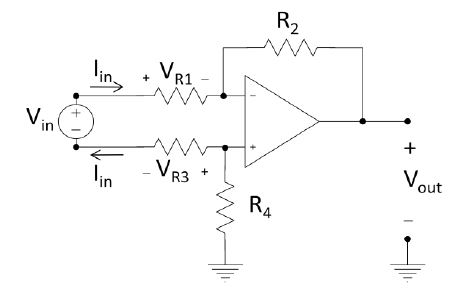
\includegraphics[width=0.5\textwidth]{billeder/Hardware/differensmodstand.JPG}
	\caption{illustration af differensforstærkerens indgangsmodstand}
	\label{fig:differensmodstand}
\end{figure}
\begin{align}
 R_{in} =V_{in}/I_{in}
 \label{eq:differensmodstand}
 \end{align}
I den ideelle verden antages det, at spændingsforskellen i mellem indgangsterminalerne er nul derfor kan der skrives vha. Kirchoffs spændingslov skrives i \ref{eq:differensmodstand2}
\begin{align}
 V_{R3}-V_{in}+V_{R1}=0=>V_{in}=V_{R3}+V_{R3}=I_{in}(R1+R3)=>R_{in}=\frac{V_{in}}{I_{in}=R1+R2}
 \label{eq:differensmodstand2}
 \end{align}
 I \ref{eq:differensmodstand2} viser det sig at indgangsmodstanden er beskrevet ved modstandene i det omkring liggende kredsløb. Hvilket giver anledning til at vælge så høje modstande som mulige, men store modstande øger risikoen for støj i kredsløbet. Det betyder at ønsket ikke kan opfyldes, med blot en differensforstærker


Punkt 3, en høj undertrykkelse af støj. Støj kan skyldes rigtig mange ting, en typiske støjkomponent er 50 Hz brum. 50 Hz brum fremkommer ofte, da støjen skyldes de omkring liggende EL installationer, hvor der foregår en elektromagnetisk kobling. men når der benyttes en differensforstærker, kan common mode støjen undertrykkes. Common mode støj er indstrålet støj der kommer på begge ledninger til differensforstærkeren. Det er differensforstærkeren god til at fra sorterer, fordi den trækker de to input fra hinanden. Det vil sige at hvis støjen er ens på de to ledninger, vil den differentiere den samme værdi fra hinanden hvilket vil give 0. en illustration af dette kan ses på figur \ref{fig:differensNoise} 
\begin{figure}[H]
	\centering
	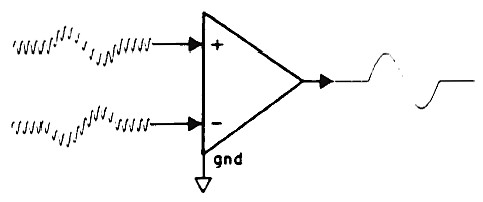
\includegraphics[width=0.5\textwidth]{billeder/Hardware/differensnoise.jpg}
	\caption{Illustration af differensforstærkerens common mode støj undertrykkelse}
	\label{fig:differensNoise}
\end{figure}

Punkt 4, en simpel forstærkning. Med det over stående kredsløb, kan en simpel forstærkning ikke opnås. Det kan det ikke da det kræver at R2 divideret med R1 er lig med R4 divideret med R3. Hvilket vil være umuligt da modstande har en tolerancer for, hvor præcise de er.

For at opfylde de ønskede egenskaber skal differensforstærkeren modificeres. For at sikres en høj indgangsmodstand kan en spændingsfølger benyttes, som har til formål at forstærke en-til-en. Det vil sige at den i teorien har samme udgangsspænding som indgangsspændingen. se figur \ref{fig:bufferamp} for en illustration, denne sættes på begge outputs fra vægtcellen.
\begin{figure}[H]
	\centering
	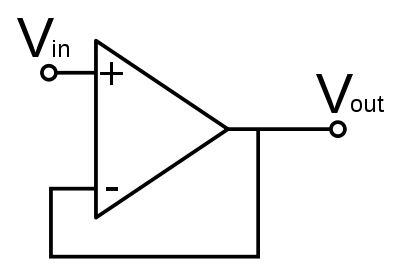
\includegraphics[width=0.5\textwidth]{billeder/Hardware/bufferamp.png}
	\caption{illustration af spændingsfølger}
	\label{fig:bufferamp}
\end{figure}
Med en spændingsfølger opnås der en høj indgangsmodstand, men signalet er stadig differentielt og uden forstærkning. Derfor indsættes der 3 modstande som vist i \ref{fig:bufferampmedgain}\citep{ASBbog}s.200
\begin{figure}[H]
	\centering
	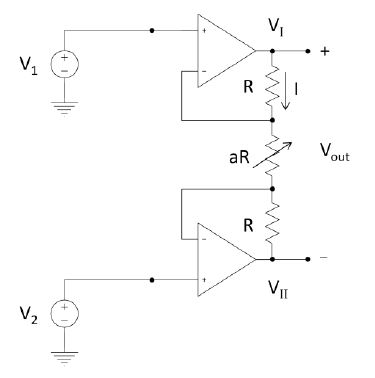
\includegraphics[width=0.5\textwidth]{billeder/Hardware/bufferampgain.JPG}
	\caption{illustration af spændingsfølger med gain}
	\label{fig:bufferampmedgain}
\end{figure}
Ved brug af KVL og KCL kan forstærkningen skrives som i \ref{eq:gain}, hvor $A_{d}$ er forstærkningen og $R_{a}$ er modstanden i midten. Dette gør forstærkningen simpel fordi der kun skal ændres en modstand. 
\begin{align}
 A_{d}=1+\frac{R+R}{R_{a}}
 \label{eq:gain}
 \end{align}
 Til at opfylde ønskerne om undertrykkelse af støj og et single ended output kan differensforstærkeren sættes efter spændingsfølgerne med forstærker trinet. Hvilket får kredsløbet til at se ud som vist i \ref{fig:bufferampmedgaindifferens}
 
 \begin{figure}[H]
	\centering
	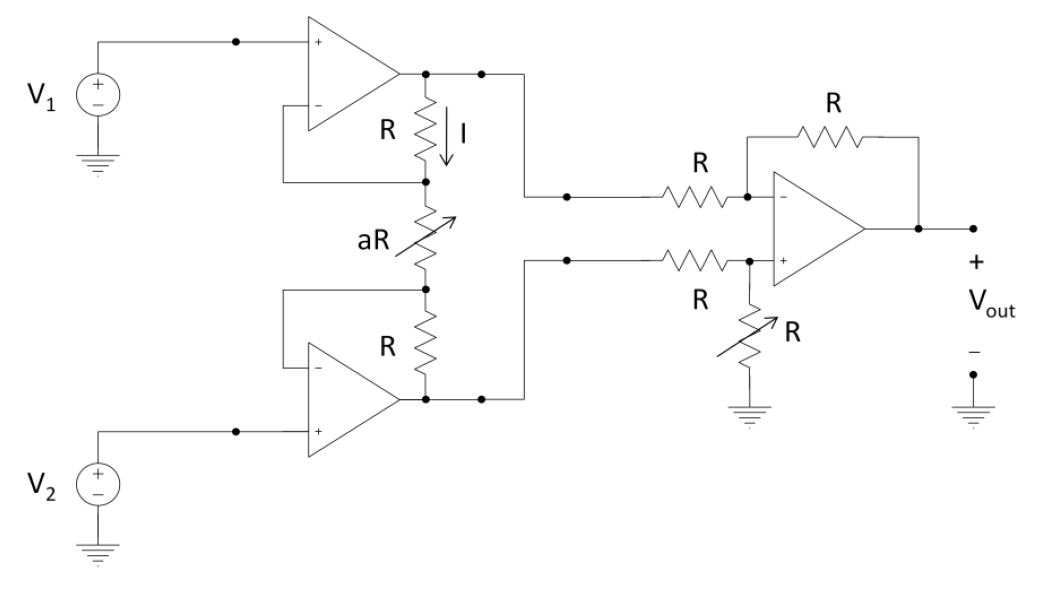
\includegraphics[width=0.5\textwidth]{billeder/Hardware/bufferampgaindifferens.JPG}
	\caption{illustration af spændingsfølger med gain og differensforstærker}
	\label{fig:bufferampmedgaindifferens}
\end{figure}

Ligning \ref{eq:instru} viser overføringsfunktionen for diagrammet i \ref{fig:bufferampmedgaindifferens}.

\begin{align}
 V_{out}=(V_{2}-V_{1})*(1+\frac{R+R}{R_{a}})
 \label{eq:instru}
 \end{align} 
 
Kredsløbet på figur \ref{fig:bufferampmedgaindifferens} kaldes en instrumentationsforstærker, hvilket der i projeket er indkøbt da den lever op til de ønskede egenskaber og er mere præcis end at lave kredsløbet selv. Den indkøbte instrumentationsforstærker hedder INA114, som har kredsløbet- og pinkonfiguration vist på \ref{fig:INA114diagram} og \ref{fig:INA114Pin}\footnote{hentet fra databladet fra INA114}
 
 \begin{figure}[htbp] \centering
\begin{minipage}[b]{0.48\textwidth} \centering
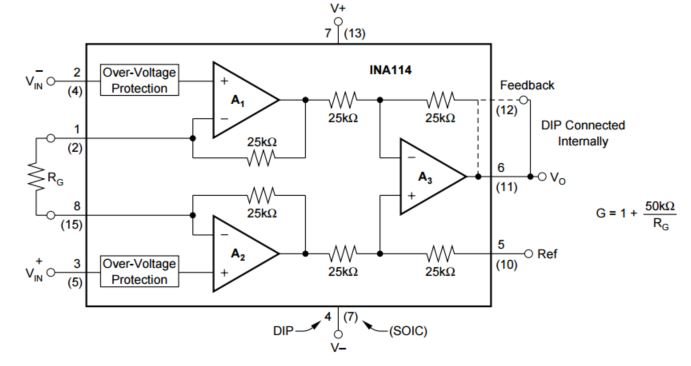
\includegraphics[width=1.00\textwidth]{billeder/Hardware/INA114diagram.JPG} % Left picture
\end{minipage} \hfill
\begin{minipage}[b]{0.48\textwidth} \centering
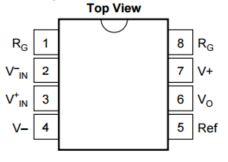
\includegraphics[width=1.00\textwidth]{billeder/Hardware/pinkonfig.JPG} % Right picture
\end{minipage} \\ % Captions og labels
\begin{minipage}[t]{0.48\textwidth}
\caption{INA114 diagram} % Left caption and label
\label{fig:INA114diagram}
\end{minipage} \hfill
\begin{minipage}[t]{0.48\textwidth}
\caption{pin konfiguration af INA114 8pin } % Right caption and label
\label{fig:INA114Pin}
\end{minipage}
\end{figure}

I databladet \ref{bilag:INA114} til INA114 ses det at den har en CMRR på 115dB, ved et gain på 1000 og en indgangsmodstand på 10G$\Omega$. Forstærkningen kan regnes ud fra formlen i databladet \ref{eq:gainina1}
\begin{align}
 G=(1+\frac{50K\Omega}{R_{G}})
 \label{eq:gainina1}
 \end{align} 
 I dette projekt skal der bruges et gain på $\frac{4,9V}{5mV}=980$, 4,9V for ikke at komme i mætning på arduinoens ADC og 5mV da det er den maksimale spænding vægtcellen kan give, ved 5V forsyning.
 \begin{align}
 R_{G}=\frac{50K\Omega}{980-1}=51\Omega
 \label{eq:gainina2}
 \end{align}
Med et gain på 980 giver en $NY_{Maksimalespænding}=980*5mV=4,9V \pm0,147V$, dvs at der nu er en opløsning på
\begin{align}
 \frac{1000g}{trin}=\frac{1000g}{1024}=0,977g/trin=>0,977*\frac{1024}{5V}=200g/V \pm30g
 \label{eq:gainina3}
 \end{align}
 
 Kredsløbet for INA114 og vægtcellen til arduinoen kan ses på figur \ref{fig:loadcelldiagram}
 
  \begin{figure}[H]
	\centering
	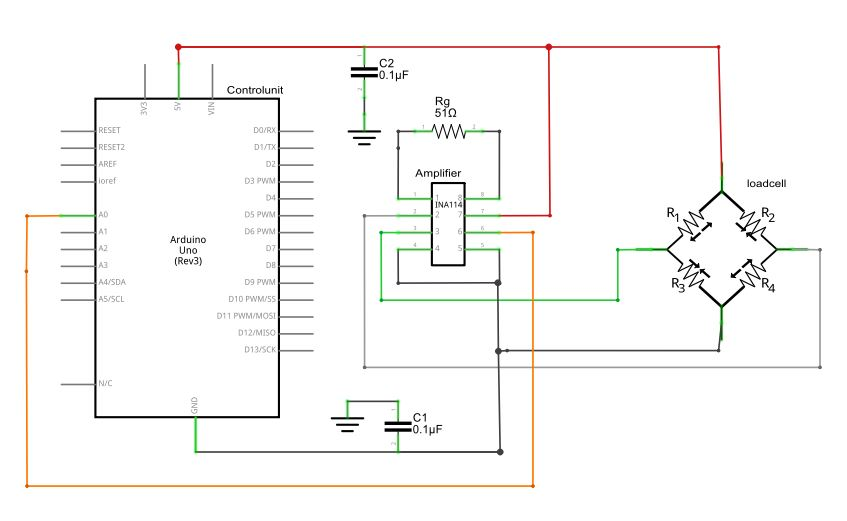
\includegraphics[width=0.9\textwidth]{billeder/Hardware/diagrammer/loadcelldiagram.JPG}
	\caption{Diagram for arduino, INA114 og vægtcelle}
	\label{fig:loadcelldiagram}
\end{figure}

\subsubsection{Enhedstest af vægtcelle }

Efter at diagrammet er fastlagt, testes forbindelserne nu på et \textit{fumlebræt} se figur \ref{fig:loadcelltest} for test opstilling

  \begin{figure}[H]
	\centering
	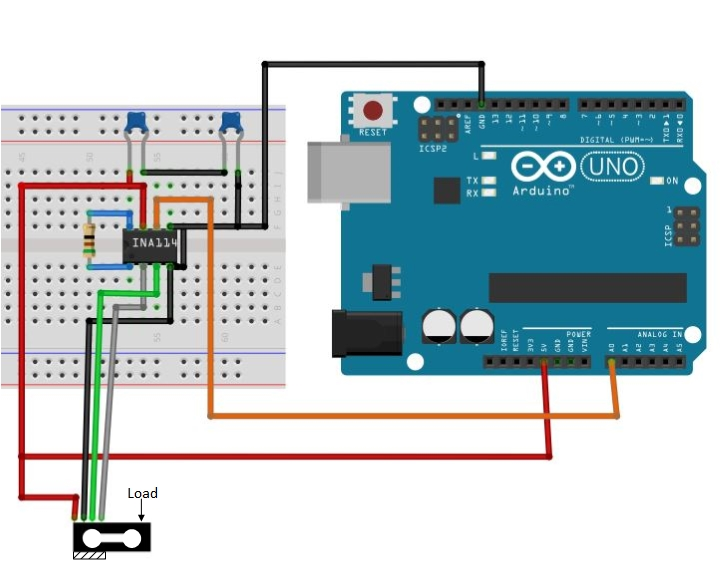
\includegraphics[width=0.9\textwidth]{billeder/Hardware/diagrammer/Drawing1.jpg}
	\caption{Test opstilling for vægtcelle}
	\label{fig:loadcelltest}
\end{figure}
De primære dele af test koden har været  \textit{sensorValue = analogRead(A0);} og \textit{Serial.println(sensorValue);}, hvor ved at inputtet på \textit{A0} er læst i \textit{serial monitor} som vist på figur \ref{fig:loadcell_test} ved langsom tømning af beholderen.

\begin{figure}[H]
	\centering
	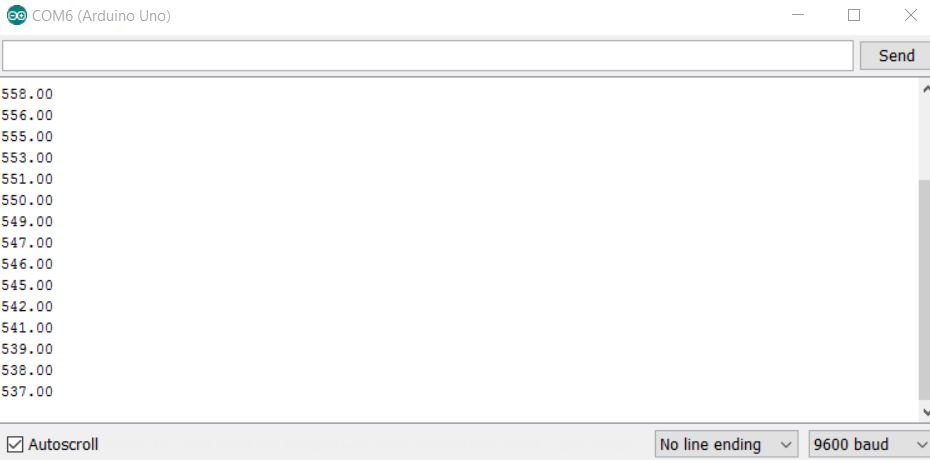
\includegraphics[width=0.9\textwidth]{billeder/Hardware/diagrammer/loadcellunittestbits.JPG}
	\caption{Værdier fra A0 i \textit{serial monitor}}
	\label{fig:loadcell_test}
\end{figure}

 Se bilag \ref{bilag:TKloadcell} for at se hele koden til testen. Til enhedstesten er der brugt et voltmeter til, at måle udgangsspændingen på INA114 for, at se om arduinoens ADC læste rigtigt. Til at sammenligne med voltmeteret, blev \ref{eq:trintilvolt} brugt til at konvertere ADC'ens bits værdi om til spænding.
 
 \begin{align}
 analogRead(A_0)*\frac{5}{1024}=\text{spænding i volt}
 \label{eq:trintilvolt}
 \end{align}
Testopstilling af vægtcellen ser ud som på \ref{fig:loadcell_mont} med celleopløsningsbeholderen. I softwaren kræves det en kalibrering for at vægtcellen er præcis, dette er implementeret i afsnit \ref{subsub:softwareloadcell}.
 
 \begin{figure}[H]
	\centering
	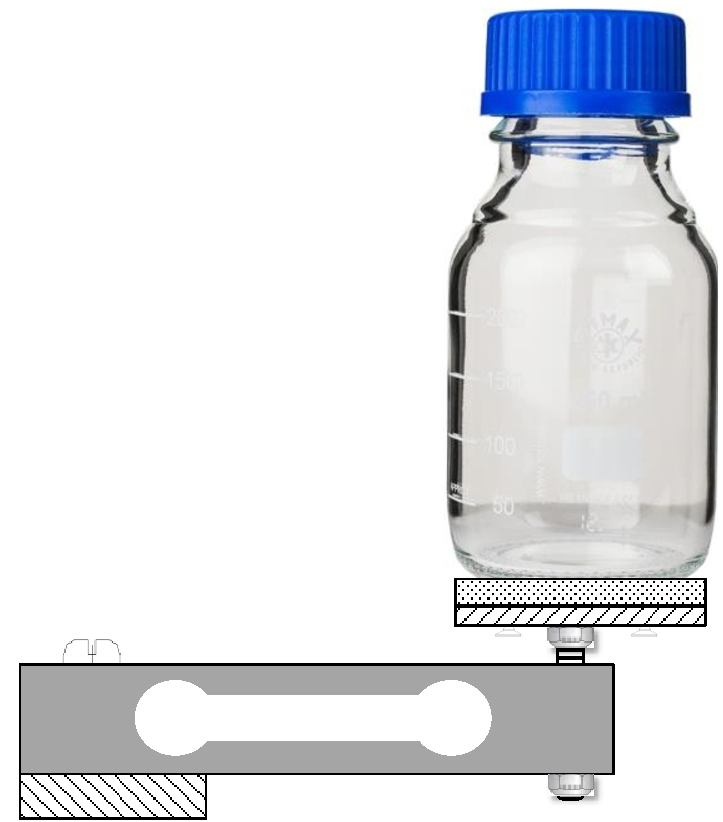
\includegraphics[width=0.5\textwidth]{billeder/Hardware/diagrammer/loadcell_montering.pdf}
	\caption{Illustration af opstilling med vægtcelle og celleopløsningsbeholder}
	\label{fig:loadcell_mont}
\end{figure}

 \subsection{Pumpe}
 Pumpen består af en DC motor og ud fra databladet kan det ses at den skal bruge 6VDC og 0.6A for at køre. Da arduinoen langt fra kan leverer den nødvendige strøm, til at drive motoren. skal der bruges en motordriver med en ekstern strømforsyning.
 \subsubsection{Motordriver}
 Motordriveren består i dette projekt af en L293D, som enten kan drive 4 motorer den ene vej, 2 motorer i begge retninger eller i dette tilfælde en vakuum pumpe og en magnetventil. se figur \ref{fig:L293DInterndiagram} for L293D interne kredsløb diagram. 
   \begin{figure}[H]
	\centering
	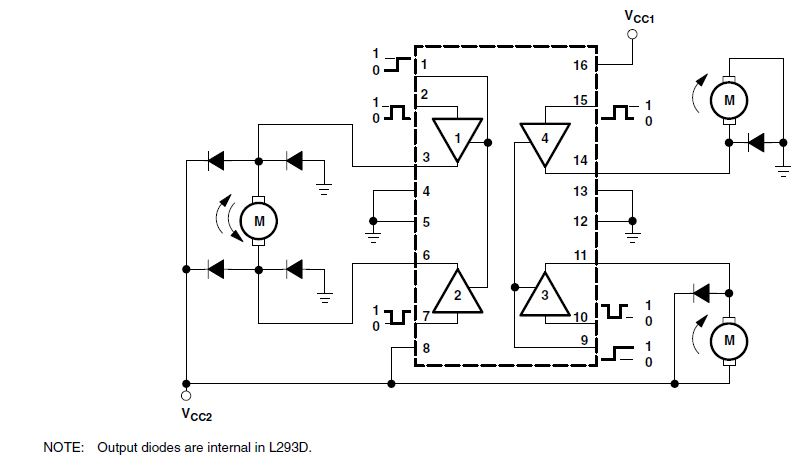
\includegraphics[width=0.9\textwidth]{billeder/Hardware/diagrammer/L293intern.JPG}
	\caption{Intern kredsløbsdiagram for L293D}
	\label{fig:L293DInterndiagram}
\end{figure}
Motordriverens opgaver er forsyne motoren, i sin simple form skal L293D tage signalet fra arduinoen, analysere det og give et tilsvarende signal fra strømforsyning til motoren.
\subsubsection{Hastighedscontrol af pumpe}
Da det er svært at finde en pumpe der præcis opfylder kravet til hastigheden i dette system, grundet de 30 øer i minuttet(\ref{subsec:Kvalitetskrav}.1)
\begin{align}
\frac{\text{Opløsningsstørelse}}{\text{Antal øer i opløsning}} = \frac{150}{200}*30 = 22,5ml/min
\label{eg:ohastighed}
\end{align}(\textit{jf. Søren Gregersen})
Der er 3 primært metoder til, at styre hastigheden på en DC-motor \citep{ELengbog}s.810.

1. Indsætte modstand i kredsløbet før motoren er koblet til.
Denne metode kan bruge på alle typer af motorer. I den simple forstand kan variabel modstand sættes i serie med motoren for, at styre hastigheden. Ulemperne ved dette kredsløb er at ,forbruget vil være ens ved den højeste hastighed og den laveste. Det vil det fordi modstanden vil blot omsætte energien til varme, hvilket vil være splid af energi. Se figur \ref{fig:motormodstand}, princippet er baseret på KVL.

\begin{figure}[H]
	\centering
	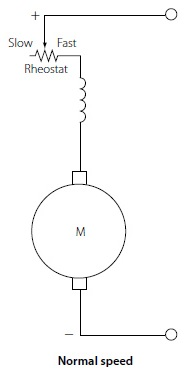
\includegraphics[width=0.3\textwidth]{billeder/Hardware/motormodstand.jpg}
	\caption{Kredsløbsdiagram for Motor med variablemodstand}
	\label{fig:motormodstand}
\end{figure}

2. Variere strømmen der tilføres motoren, hvor spændingen holdes konstant.
Denne metode minder om den overstående, men i stedet for serie kobles den variable modstand parrallet, som det kan ses på figur \ref{fig:motorcurrent}. Ulempen ved dette kredsløbt er at når motoren skal køre ved lav hastighed, er modstanden lille og derved tæt på en kortslutning derfor er det vigtigt, at kredsløbet er designet rigtigt. Princippet er baseret på KCL.

\begin{figure}[H]
	\centering
	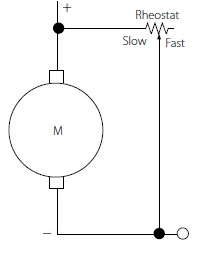
\includegraphics[width=0.3\textwidth]{billeder/Hardware/motorcurrent.jpg}
	\caption{Kredsløbsdiagram for Motor med variable strøm}
	\label{fig:motorcurrent}
\end{figure}

\fxnote{hvis tiden er til det, kan der uddybes med generel motor teori som opbygning mm. Derud over kunne der sagtens lave nogle formler også til generelle motorer, så som moment mm.}


3. Varierer spændingen der tilføres motoren periodevis, hvor strømmen holdes konstant.
Konceptet i denne metode er at have en konstant forsyning, som i sin simple forstand slukkes og tændes for. Dvs. at der sidder en kontakt i mellem strømforsyningen og motoren, der tændes og slukkes. Kredsløbet for dette kan stilles op som figur \ref{fig:motorkontakt} og giver et signal som på figur \ref{fig:onoffwave}

 \begin{figure}[htbp] \centering
\begin{minipage}[b]{0.48\textwidth} \centering
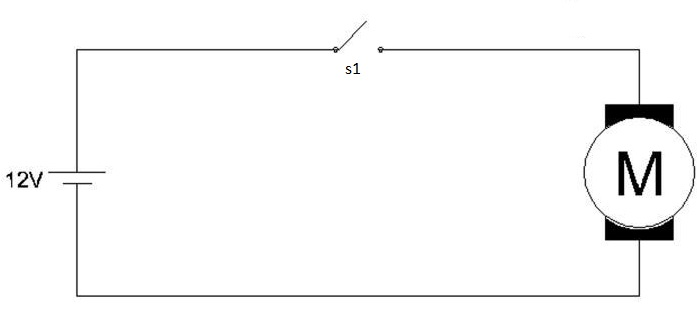
\includegraphics[width=1.00\textwidth]{billeder/Hardware/motorkontakt.jpg} % Left picture
\end{minipage} \hfill
\begin{minipage}[b]{0.48\textwidth} \centering
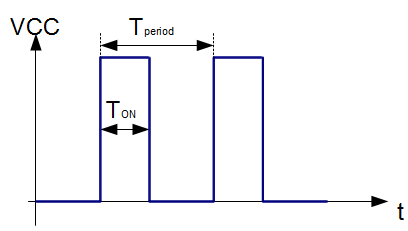
\includegraphics[width=1.00\textwidth]{billeder/Hardware/onoffwave.jpg} % Right picture
\end{minipage} \\ % Captions og labels
\begin{minipage}[t]{0.48\textwidth}
\caption{Kredsløbsdiagram for Motor med en kontakt} % Left caption and label
\label{fig:motorkontakt}
\end{minipage} \hfill
\begin{minipage}[t]{0.48\textwidth}
\caption{Motorsignal ved periodevis spænding } % Right caption and label
\label{fig:onoffwave}
\end{minipage}
\end{figure}
Åbningstiden $T_{on}$ er der hvor kontakten er tændt, $T_{period}$ er perioden som kontakten åbner og lukker. Den gennemsnitlige spænding kan regnes ud ved \ref{eq:VT}

\begin{align}
V_T=V_S \frac{T_{on}}{T_{period}}
\label{eq:VT}
\end{align}
Ud fra overstående formel (\ref{eq:VT}) ses det, at gennemsnit spændingen og derved også hastigheden på motoren styres ved $T_{on}$ altså hvor langtid kontakten er tændt. Denne form for styring af en motor, kaldes også pulse width modulation.



\paragraph{Pulse width modulation} \phantom{mmmmmmmmmmmmmmmmmkkkkkkkkkkkkkkkkkkkkkkkkkkkkkkkkmmmmmmmmmmmmmmmmmmmmmm}

Pulse width modulation(PWM) er en meget brugt metode som kan bruges til, at styre hastigheden på en DC motor. Dette gøres ved at tænde og slukke for en digital udgang. Det er duty cyklussen der får hastigheden til at varierer, dvs. at det er tiden hvor det firkantede signal er "højt" der bestemmer hastigheden. Da strømforsyningen er 12V og motoren kun kan tåle 6V, betyder det at duty cyklussen ikke må overstige 50\%, da det vil give en højere gennemsnits spænding end 6V, hvilket er motorens maksimale spænding. Se figur \ref{fig:pwmsignal} for illustration af PWM duty cyklusser og gennemsnit spændinger. PWM styring kan bruges til blandt andet dæmning af dioder, generering af lydsignaler og styring af motorer \fxnote{højere fagligt sprog og niveau og nogle gode referencer}. 

 \begin{figure}[H]
	\centering
	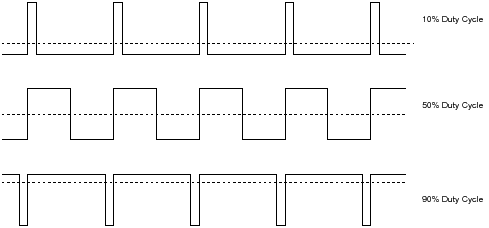
\includegraphics[width=0.8\textwidth]{billeder/Hardware/pwm.png}
	\caption{PWM duty cyklusser med gennemsnits spændinger}
	\label{fig:pwmsignal}
\end{figure}

Der er flere metoder, hvor dette kan implementeres vha. arduinoen. Den mest simple metode er $analogWrite(pin, dutyCycle);$ hvor dutycycle er en værdi mellem 0 og 255 og pin er en af de digital udgange med PWM. Dette er simpelt, men der er ingen control over frekvens mm. 

Manuel PWM implementering er en anden metode, der kan implementeres således:

\begin{lstlisting}
void setup()
{
  pinMode(13, OUTPUT);
}

void loop()
{
  digitalWrite(13, HIGH);
  delayMicroseconds(100); // Approximately 10% duty cycle @ 1KHz
  digitalWrite(13, LOW);
  delayMicroseconds(1000 - 100);
}
\end{lstlisting}

Her sættes pin 13 til \textit{høj}, hvor efter der ventes 100 mikro sekunder. Derefter sættes pin 13 \textit{lav} og der ventes 900 mikro sekunder. Ved denne metode kan alle digitale udgange bruges og ikke kun dem med PWM. Dog er processeren brugt hele tiden da den også bruges når der ventes. Det vil sige at den ikke kan bruges til andet samtidigt, hvilket ikke kan bruges i projektet.
Microcontrolleren der sidder på arduinoen indeholder 3 timere, som kan bruges til PWM generering.  Måden dette virker på er at timeren går fra 0 til 255, hvis $Timer=0$ sættes outputtet højt, hvor den tæller til enten 255 og slukker hvilket vil skabe en duty cyklus på 100\%. Derfor kan der defineres en værdi hvor der slukkes mellem 0 og 255. Ydermere findes der scalar (1, 8, 64, 256 eller 1024 som divideres med arduinoens clock frekvens. Alt dette konfigureres ved bits i registre (TCCRnA og TCCRnB) på microcontrolleren. Et eksempel på dette kunne være: 

\begin{lstlisting}
void setup()
{
pinMode(3, OUTPUT);
  pinMode(11, OUTPUT);
  TCCR2A = _BV(COM2A1) | _BV(COM2B1) | _BV(WGM21) | _BV(WGM20);
  TCCR2B = _BV(CS22);
  OCR2A = 180;
  OCR2B = 50;
\end{lstlisting}

Ved overstående kode vil der være en duty cyklus på output A da være $$\frac{180+1}{256}*100=70,7\%$$ og en PWM frekvens på     
  $$\frac{16MHz}{64/256}=976.6Hz$$. Output B vil have en duty cyklus på $$\frac{50+1}{256}*100=19.9 \%$$ og den samme frekvens. Den sidst nævnte metode, er den metode hvor der er mest kontrol over PWM signalet. Derfor bruges denne i dette projekt.
  
For at lysdioderne får deres ønskede spænding, er det nødvendigt med modstande foran dem. Modstandene kan beregnes på følgende måde. 
\begin{align}
R=\frac{V_{source}-V_{lysdiode}}{I_{lysdiode}}=\frac{6-3.2}{20mA}=140\Omega
\label{eq:modstandLEDmotor}
\end{align} 
Dette giver en effekt afsætning i modstandene på $(V_{source}-V_{lysdiode}*I_{lysdiode}=2,8*20mA=0,056W)$ hvilket giver grund for at 0.33W modstande er passende.


\subsubsection{Enhedstest af motor og motordriver}
\label{subsubsec:enhedstestmotor}
 På figur \ref{fig:motordriverdiagram} kan ledningsdiagrammet til motordriver med motor og frem og tilbage lysdioder observeres. Med opsætningen kan retningen på motoren bestemmes ved, hvilken en af udgangene der sættes til lav(0V). Hvor den modsatte udgang konfigureres til PWM. Gøres det modsat kører motoren den modsatte vej. På figur \ref{fig:Motorbreadboard} ses kredsløbet monteret ved enhedstesten på et \textit{fumlebræt}.
 
 \begin{figure}[H]
	\centering
	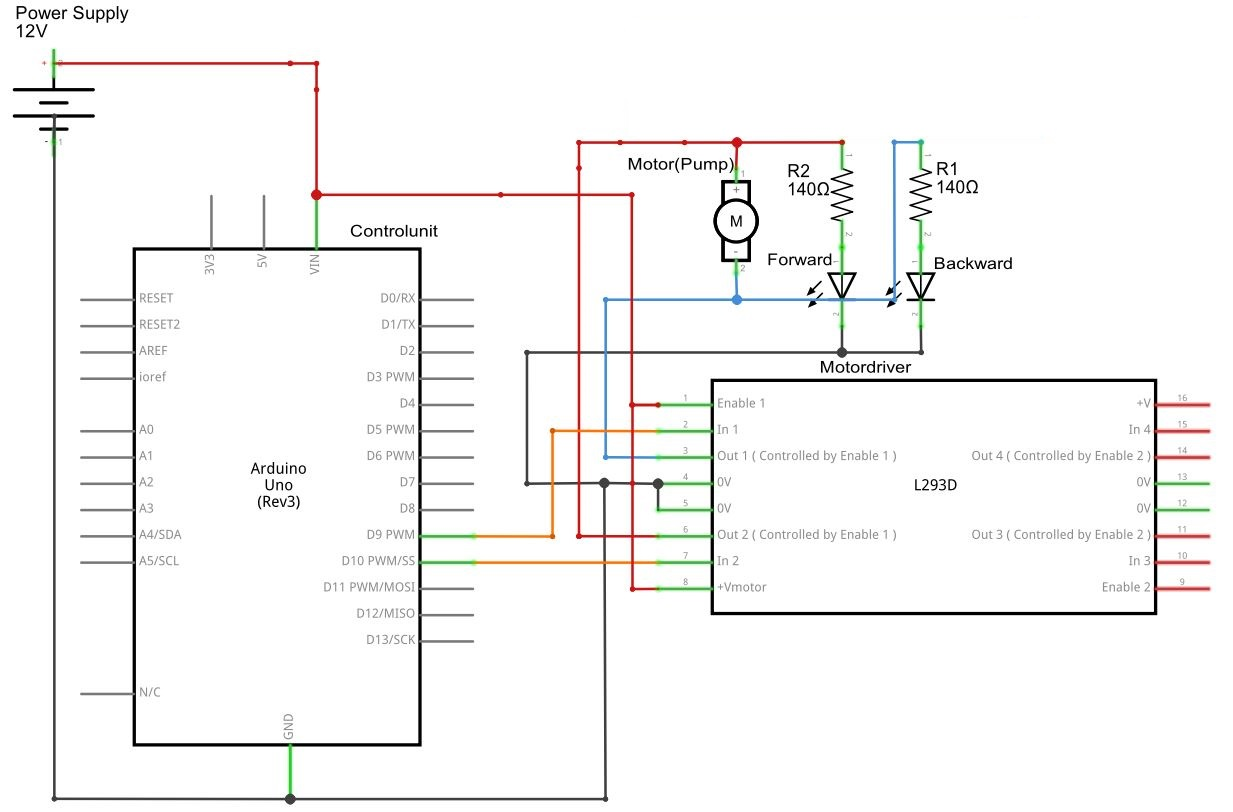
\includegraphics[width=1\textwidth]{billeder/Hardware/diagrammer/motordiagram.JPG}
	\caption{Kredsløbsdiagram for motor og motordriver}
	\label{fig:motordriverdiagram}
\end{figure}

 \begin{figure}[H]
	\centering
	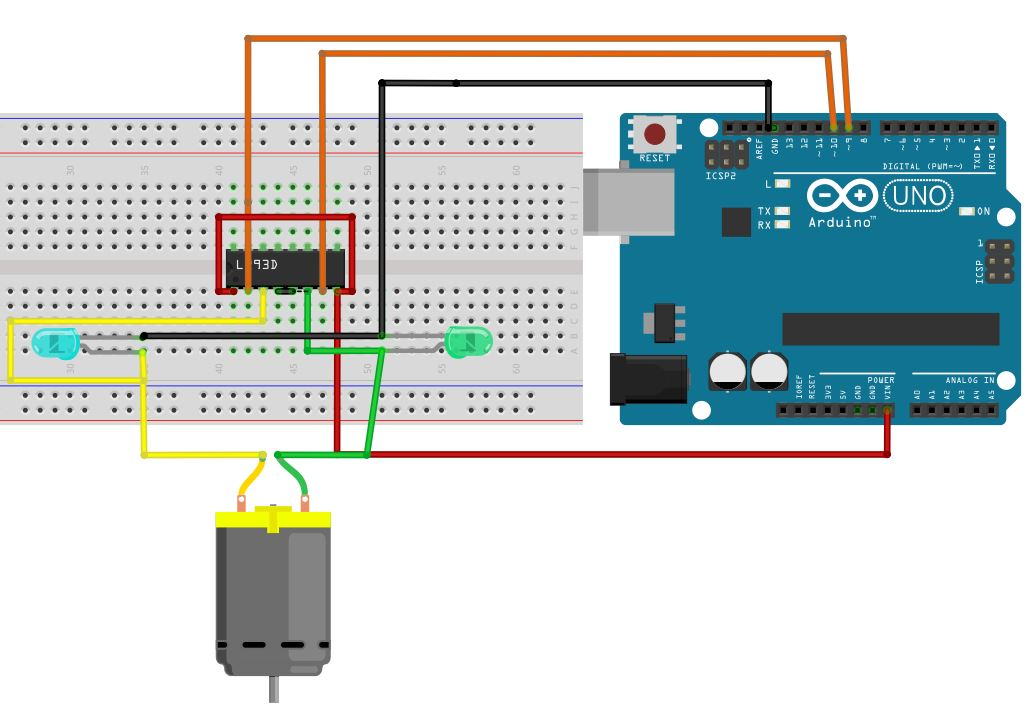
\includegraphics[width=1\textwidth]{billeder/Hardware/diagrammer/Motorbreadboard.JPG}
	\caption{Illustration af opstilling med motor(pumpe), motordriver og arduino}
	\label{fig:Motorbreadboard}
\end{figure}

For at teste motordriverens evne til at lave PWM med 12 volt, er PWM signalet fra arduinoen og motordriveren sammenlignet med hinanden vha. et oscilloskop. Billeder fra denne test er vist på  billederne \ref{fig:25PWM}, \ref{fig:50PWM}, \ref{fig:75PWM} og \ref{fig:100PWM} den høje gule graf er fra motordriveren og den grønne lave graf er fra arduinoen.

\newpage

 \begin{figure}[htbp] \centering
\begin{minipage}[b]{0.48\textwidth} \centering
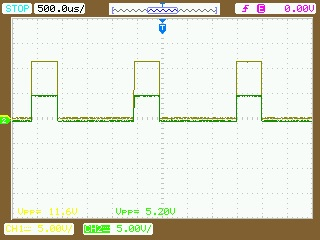
\includegraphics[width=1.00\textwidth]{billeder/Hardware/motor25PWM.jpg} % Left picture
\end{minipage} \hfill
\begin{minipage}[b]{0.48\textwidth} \centering
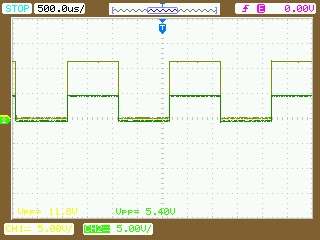
\includegraphics[width=1.00\textwidth]{billeder/Hardware/motor50PWM.jpg} % Right picture
\end{minipage} \\ % Captions og labels
\begin{minipage}[t]{0.48\textwidth}
\caption{Arduino og motordriver med 25$\%$ PWM} % Left caption and label
\label{fig:25PWM}
\end{minipage} \hfill
\begin{minipage}[t]{0.48\textwidth}
\caption{Arduino og motordriver med 50$\%$ PWM} % Right caption and label
\label{fig:50PWM}
\end{minipage}
\end{figure}

 \begin{figure}[htbp] \centering
\begin{minipage}[b]{0.48\textwidth} \centering
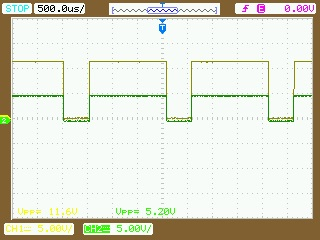
\includegraphics[width=1.00\textwidth]{billeder/Hardware/motor75PWM.jpg} % Left picture
\end{minipage} \hfill
\begin{minipage}[b]{0.48\textwidth} \centering
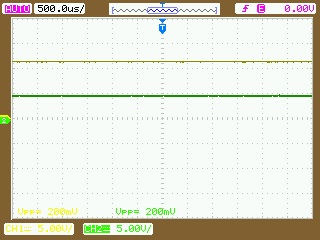
\includegraphics[width=1.00\textwidth]{billeder/Hardware/motor100PWM.jpg} % Right picture
\end{minipage} \\ % Captions og labels
\begin{minipage}[t]{0.48\textwidth}
\caption{Arduino og motordriver med 75$\%$ PWM} % Left caption and label
\label{fig:75PWM}
\end{minipage} \hfill
\begin{minipage}[t]{0.48\textwidth}
\caption{Arduino og motordriver med 100$\%$ PWM} % Right caption and label
\label{fig:100PWM}
\end{minipage}
\end{figure}

De elementære funktioner, som er brugt til test koden er \textit{digitalWrite(9, LOW);} og \textit{analogWrite(10, 127);}. se hele testkoden i bilag \ref{bilag:TKpumpe}

\newpage

 \subsection{Ventil}
 En magnetventil virker på den måde at den består af en spole, der danner et magnetfelt når der bliver påsat spænding og derved trækker et stempel til sig. Det får ventilen til at åbne ved hjælp af en membran. En trevejs magnetventil, som den brugte i dette projekt virker på samme måde. Men hvor skifter position er designet så der altid er en åben. Derfor vil opløsningen løbe ud i wastebeholderen når der ikke er en langerhanske ø, men kommer der en vil den skifte position, hvorved de bliver frasorteret. Se figur \ref{fig:ventilpos} for en illustration af en 3 vejs magnetventil.

\begin{figure}[H]
	\centering
	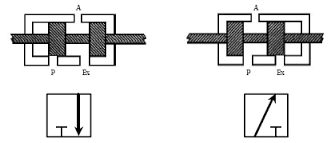
\includegraphics[width=0.5\textwidth]{billeder/Hardware/ventil.png}
	\caption{Magnetventil position}
	\label{fig:ventilpos}
\end{figure}  
For at sorteringen af langerhanske øer sker, kræver det en beregning af hastigheden det tager for en langerhansk ø, at komme fra kameraet til ventilen. Det kan estimeres ud fra at beregne volumenet af slangen, i mellem kameraet og ventil ref(volume).
\begin{align}
V=\pi*r^2*h=\pi*\frac{\SI{51}{\micro\metre}}{2}*5cm=0,04ml
\end{align}
 Det vil sige at med et flow på 22,5ml/min, som er beregnet ud fra formlen \ref{eg:ohastighed}. Her ud fra kan det beregnes tiden fra kamera til ventil. 
 \begin{align}
\frac{22,5}{60}*0,04ml=0.106\text{sekunder}=106ms
\end{align}

Yderligere skal ventilen åbne lidt før og lukke lidt efter. Derfor skal der også være en tid for, hvor lang tid ventilen skal være åben, dette bør testes i en enhedstest af ventilen.

Ligesom ved motoren er det også her nødvendigt, at sætte en modstand foran lysdioden. Modstanden er af samme type som til kameralyset se \ref{subsec:kameralys} for beregninger for dem. 

\newpage
 På figur \ref{fig:ventildiagram} kan der ses et diagram over arduinoen, motordriveren og ventilen.

\begin{figure}[H]
	\centering
	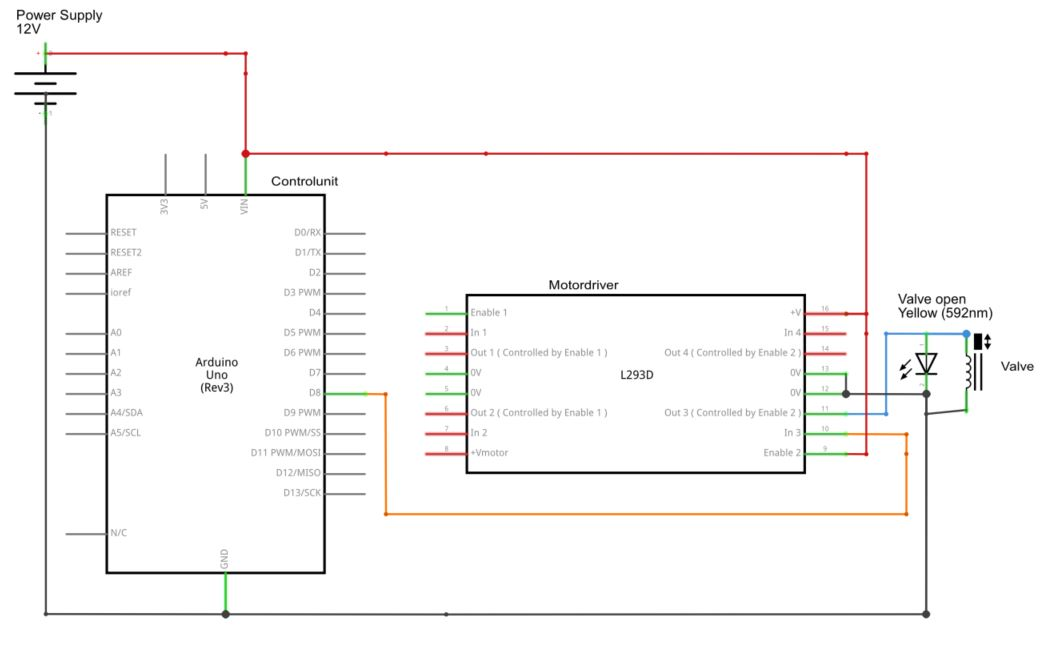
\includegraphics[width=1\textwidth]{billeder/Hardware/diagrammer/ventildiagram.JPG}
	\caption{Kredsløbsdiagram for ventil}
	\label{fig:ventildiagram}
\end{figure} 
\newpage
\subsubsection{Enhedstest for ventil}
På figur \ref{fig:ventilbreadboard} er det illustreret hvordan testopstilling er sat op på et \textit{fumlebræt}. I test koden er der hovedsagligt brugt \textit{digitalWrite(8, LOW);} og \textit{digitalWrite(8, HIGH);}, hvorved arduinoen sætter udgangen lav(0V) og høj(5V). Motordriveren bruger signalet til det at give ventilen 12V når den er høj. Se bilag \ref{bilag:TKventil} for hele testkoden

\begin{figure}[H]
	\centering
	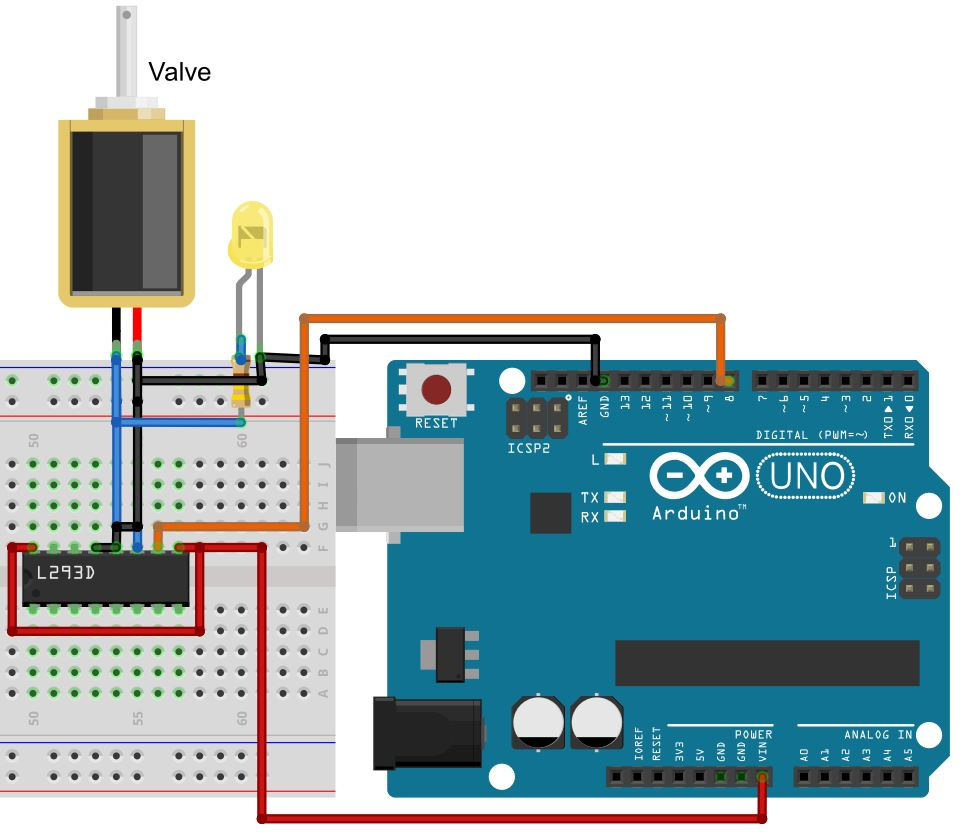
\includegraphics[width=1\textwidth]{billeder/Hardware/diagrammer/Ventilbreadboard.JPG}
	\caption{Illustration af testopstilling med ventil og motordriver}
	\label{fig:ventilbreadboard}
\end{figure} 
 
\newpage
 \subsection{Kameralys}
 \label{subsec:kameralys}
 Kameralyset skal kunne variere, da operatøren skal kunne indstille lyset for den bedst mulige opsætning. Det gøres for at kameraet har de bedste muligheder for at detekterer de langerhanske øer. Der skal sættes 4 lysdioder i en kasse, hvor kun kameralyset lyser kassen op. Kameraet skal detekterer de langerhanske øer der løber i slangen inde i kassen. Lyset implementeres for at styre lysniveauet på billederne. Da der ikke kan trækkes strøm nok ud af arduinoen, kræves det en anden forsyning til lysdioderne. Dertil udnyttes den sidste udgang i motordriveren, men da denne forsynings med 12V og lysdioder kun tåler 3.2V skal spændingen nedjusteres. Den lettest måde at gøre dette på er, at sætte lysdioderne i serie. Hvis en lysdiode bliver defekt, skabes der ingen lys til kameraet. Derfor er der valgt en løsning med modstande foran hver lysdiode. Formodstandenes værdi er beregnet ved \ref{eq:modstand}. 

\begin{align}
R=\frac{V_{source}-V_{lysdiode}}{I_{lysdiode}}=\frac{12-3.2}{20mA}=440\Omega
\label{eq:modstand}
\end{align} 
Dette giver en effekt afsætning i modstandene på $(V_{source}-V_{lysdiode}*I_{lysdiode}=8,8*20mA=0,176W)$ hvilket giver grund for at 0.33W modstande er passende.

På figur \ref{fig:LEDdiagram} vises diagrammet for Kameralyset
 
 \begin{figure}[H]
	\centering
	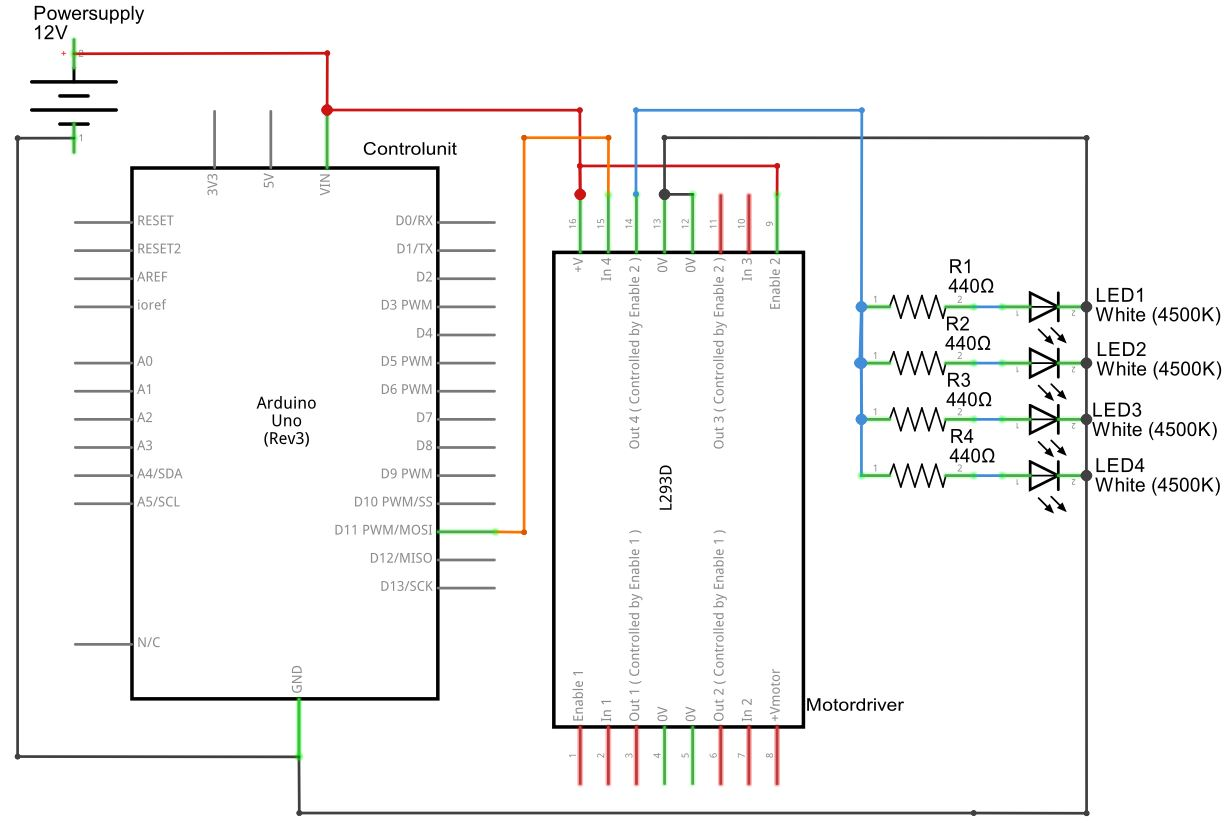
\includegraphics[width=1\textwidth]{billeder/Hardware/diagrammer/LEDdiagram.JPG}
	\caption{Kredsløbsdiagram for kameralys}
	\label{fig:LEDdiagram}
\end{figure} 

\subsubsection{Enhedstest for Kameralyset}

På figur \ref{fig:LEDbreadboard} vises testopstilling på et \textit{fumlebræt} for Kameralyset er der brugt samme test kode som til pumpen se afsnit \ref{subsubsec:enhedstestmotor}. 

\begin{figure}[H]
	\centering
	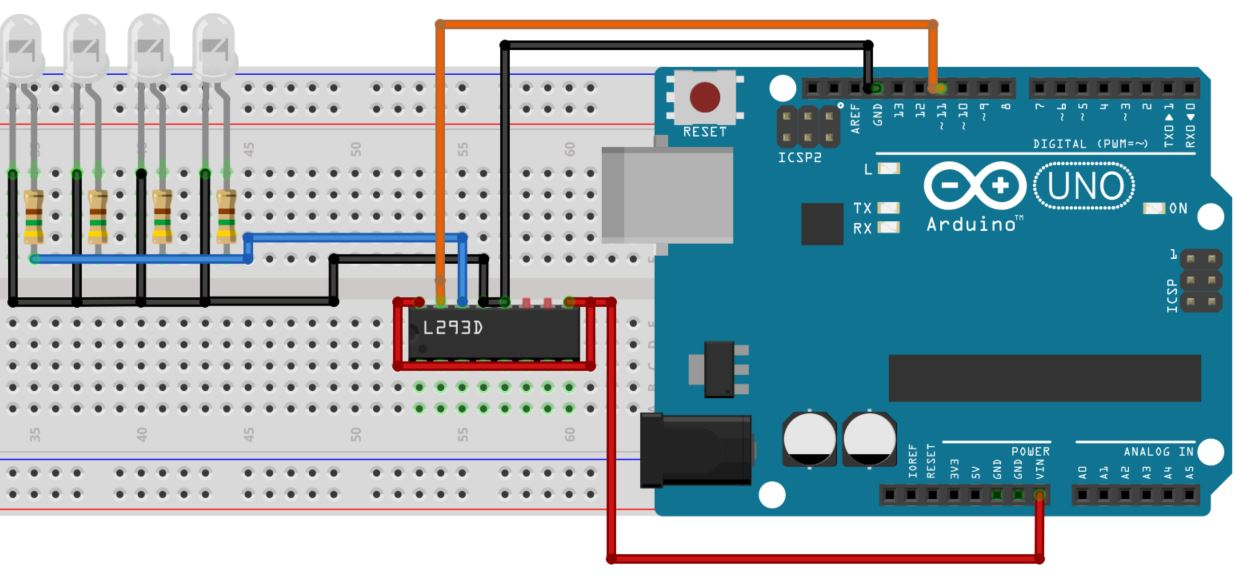
\includegraphics[width=1\textwidth]{billeder/Hardware/diagrammer/LEDbreadboard.JPG}
	\caption{Illustration af testopstilling med kameralys og motordriver}
	\label{fig:LEDbreadboard}
\end{figure}

 
\newpage 
\subsection{Ikke elektroniske dele}

IBD over hvordan dele er implementeret?

illustrationer af delene?

stykliste skal i hvertfald være der 
 
 
 
 
\subsection{Opsummering for hardware/integrationstest/PCB design} 

\begin{figure}[H]
	\centering
	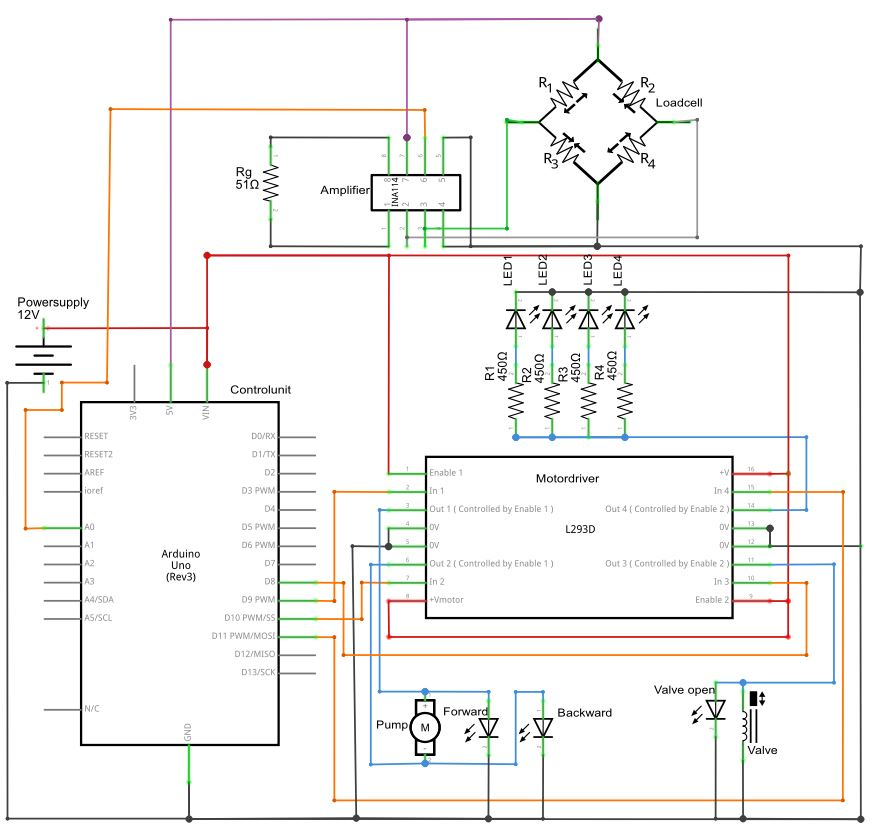
\includegraphics[width=1\textwidth]{billeder/Hardware/diagrammer/HWdiagram.JPG}
	\caption{Kredsløbsdiagram for Hardware}
	\label{fig:HWdiagram}
\end{figure}

Indsæt stykliste for alle hardware komponenter, PCB layout og beregninger her til \fxnote{mangler}
 